% Options for packages loaded elsewhere
\PassOptionsToPackage{unicode}{hyperref}
\PassOptionsToPackage{hyphens}{url}
\PassOptionsToPackage{dvipsnames,svgnames,x11names}{xcolor}
%
\documentclass[
  12pt,
]{article}

\usepackage{amsmath,amssymb}
\usepackage{iftex}
\ifPDFTeX
  \usepackage[T1]{fontenc}
  \usepackage[utf8]{inputenc}
  \usepackage{textcomp} % provide euro and other symbols
\else % if luatex or xetex
  \usepackage{unicode-math}
  \defaultfontfeatures{Scale=MatchLowercase}
  \defaultfontfeatures[\rmfamily]{Ligatures=TeX,Scale=1}
\fi
\usepackage{lmodern}
\ifPDFTeX\else  
    % xetex/luatex font selection
\fi
% Use upquote if available, for straight quotes in verbatim environments
\IfFileExists{upquote.sty}{\usepackage{upquote}}{}
\IfFileExists{microtype.sty}{% use microtype if available
  \usepackage[]{microtype}
  \UseMicrotypeSet[protrusion]{basicmath} % disable protrusion for tt fonts
}{}
\makeatletter
\@ifundefined{KOMAClassName}{% if non-KOMA class
  \IfFileExists{parskip.sty}{%
    \usepackage{parskip}
  }{% else
    \setlength{\parindent}{0pt}
    \setlength{\parskip}{6pt plus 2pt minus 1pt}}
}{% if KOMA class
  \KOMAoptions{parskip=half}}
\makeatother
\usepackage{xcolor}
\setlength{\emergencystretch}{3em} % prevent overfull lines
\setcounter{secnumdepth}{5}
% Make \paragraph and \subparagraph free-standing
\ifx\paragraph\undefined\else
  \let\oldparagraph\paragraph
  \renewcommand{\paragraph}[1]{\oldparagraph{#1}\mbox{}}
\fi
\ifx\subparagraph\undefined\else
  \let\oldsubparagraph\subparagraph
  \renewcommand{\subparagraph}[1]{\oldsubparagraph{#1}\mbox{}}
\fi


\providecommand{\tightlist}{%
  \setlength{\itemsep}{0pt}\setlength{\parskip}{0pt}}\usepackage{longtable,booktabs,array}
\usepackage{calc} % for calculating minipage widths
% Correct order of tables after \paragraph or \subparagraph
\usepackage{etoolbox}
\makeatletter
\patchcmd\longtable{\par}{\if@noskipsec\mbox{}\fi\par}{}{}
\makeatother
% Allow footnotes in longtable head/foot
\IfFileExists{footnotehyper.sty}{\usepackage{footnotehyper}}{\usepackage{footnote}}
\makesavenoteenv{longtable}
\usepackage{graphicx}
\makeatletter
\def\maxwidth{\ifdim\Gin@nat@width>\linewidth\linewidth\else\Gin@nat@width\fi}
\def\maxheight{\ifdim\Gin@nat@height>\textheight\textheight\else\Gin@nat@height\fi}
\makeatother
% Scale images if necessary, so that they will not overflow the page
% margins by default, and it is still possible to overwrite the defaults
% using explicit options in \includegraphics[width, height, ...]{}
\setkeys{Gin}{width=\maxwidth,height=\maxheight,keepaspectratio}
% Set default figure placement to htbp
\makeatletter
\def\fps@figure{htbp}
\makeatother
\newlength{\cslhangindent}
\setlength{\cslhangindent}{1.5em}
\newlength{\csllabelwidth}
\setlength{\csllabelwidth}{3em}
\newlength{\cslentryspacingunit} % times entry-spacing
\setlength{\cslentryspacingunit}{\parskip}
\newenvironment{CSLReferences}[2] % #1 hanging-ident, #2 entry spacing
 {% don't indent paragraphs
  \setlength{\parindent}{0pt}
  % turn on hanging indent if param 1 is 1
  \ifodd #1
  \let\oldpar\par
  \def\par{\hangindent=\cslhangindent\oldpar}
  \fi
  % set entry spacing
  \setlength{\parskip}{#2\cslentryspacingunit}
 }%
 {}
\usepackage{calc}
\newcommand{\CSLBlock}[1]{#1\hfill\break}
\newcommand{\CSLLeftMargin}[1]{\parbox[t]{\csllabelwidth}{#1}}
\newcommand{\CSLRightInline}[1]{\parbox[t]{\linewidth - \csllabelwidth}{#1}\break}
\newcommand{\CSLIndent}[1]{\hspace{\cslhangindent}#1}

\usepackage{geometry}
\geometry{paper=a4paper,margin=1in}
\usepackage{fontspec}
\setmainfont{Arial}
\setlength{\tabcolsep}{2pt}
\makeatletter
\makeatother
\makeatletter
\makeatother
\makeatletter
\@ifpackageloaded{caption}{}{\usepackage{caption}}
\AtBeginDocument{%
\ifdefined\contentsname
  \renewcommand*\contentsname{Table of contents}
\else
  \newcommand\contentsname{Table of contents}
\fi
\ifdefined\listfigurename
  \renewcommand*\listfigurename{List of Figures}
\else
  \newcommand\listfigurename{List of Figures}
\fi
\ifdefined\listtablename
  \renewcommand*\listtablename{List of Tables}
\else
  \newcommand\listtablename{List of Tables}
\fi
\ifdefined\figurename
  \renewcommand*\figurename{Figure}
\else
  \newcommand\figurename{Figure}
\fi
\ifdefined\tablename
  \renewcommand*\tablename{Table}
\else
  \newcommand\tablename{Table}
\fi
}
\@ifpackageloaded{float}{}{\usepackage{float}}
\floatstyle{ruled}
\@ifundefined{c@chapter}{\newfloat{codelisting}{h}{lop}}{\newfloat{codelisting}{h}{lop}[chapter]}
\floatname{codelisting}{Listing}
\newcommand*\listoflistings{\listof{codelisting}{List of Listings}}
\makeatother
\makeatletter
\@ifpackageloaded{caption}{}{\usepackage{caption}}
\@ifpackageloaded{subcaption}{}{\usepackage{subcaption}}
\makeatother
\makeatletter
\@ifpackageloaded{tcolorbox}{}{\usepackage[skins,breakable]{tcolorbox}}
\makeatother
\makeatletter
\@ifundefined{shadecolor}{\definecolor{shadecolor}{rgb}{.97, .97, .97}}
\makeatother
\makeatletter
\makeatother
\makeatletter
\makeatother
\ifLuaTeX
  \usepackage{selnolig}  % disable illegal ligatures
\fi
\IfFileExists{bookmark.sty}{\usepackage{bookmark}}{\usepackage{hyperref}}
\IfFileExists{xurl.sty}{\usepackage{xurl}}{} % add URL line breaks if available
\urlstyle{same} % disable monospaced font for URLs
\hypersetup{
  pdftitle={Mapping India in Pliny the Elder's Natural History},
  pdfauthor={Dawn, Lizao Zhuang (r0914937)},
  colorlinks=true,
  linkcolor={blue},
  filecolor={Maroon},
  citecolor={Blue},
  urlcolor={Blue},
  pdfcreator={LaTeX via pandoc}}

\title{Mapping India in Pliny the Elder's \emph{Natural History}}
\author{Dawn, Lizao Zhuang (r0914937)}
\date{}

\begin{document}
\maketitle
\begin{abstract}
this is an abstract
\end{abstract}
\ifdefined\Shaded\renewenvironment{Shaded}{\begin{tcolorbox}[breakable, boxrule=0pt, frame hidden, borderline west={3pt}{0pt}{shadecolor}, enhanced, interior hidden, sharp corners]}{\end{tcolorbox}}\fi

\renewcommand*\contentsname{Contents}
{
\hypersetup{linkcolor=}
\setcounter{tocdepth}{3}
\tableofcontents
}
\listoffigures
\listoftables
\hypertarget{sec-introduction}{%
\section{Introduction}\label{sec-introduction}}

\hypertarget{natural-history-and-its-complexity}{%
\subsection{\texorpdfstring{\emph{Natural History} and its
complexity}{Natural History and its complexity}}\label{natural-history-and-its-complexity}}

Pliny the Elder's \emph{Natural History} is widely recognized as the
earliest encyclopedia in the world, manifesting a pioneering effort in
comprehensively cataloging the vast array of human knowledge from that
era.

The work is thematically divided into 37 books, covering a diverse range
of subjects including astronomy, geography, zoology, botany, medicine,
and more. Pliny meticulously consulted a wide range of Greek and Roman
references, totaling approximately 2,000 volumes\footnote{\emph{Natural
  History} 1.5.1 (https://topostext.org/work/148)}, and interwove his
own literary interpretation or comments to the narratives.

Despite the carefully designed knowledge-ordering framework (Lao 2016),
scholars have observed a paradoxical complexity in \emph{Natural
History}, evident in its linguistic style, narrative approach, and use
of references. The work compiles inconsistent toponyms from Greek and
Latin, includes digressions in descriptions (Roller 2022), exhibits
changes in vocabularies and sentence structures (Pinkster 2005).
However, it is precisely this complexity that makes the work more
fascinating and not only a valuable source to the knowledge and
worldview of the ancient world, but also a gateway into Pliny's
conceptualization, imagination, and even the prevailing imperial
ideology.

The complexity and interconnectivity of the general structure of
\emph{Natural History} is further highlighted in different aspects by
refreshing approaches. In terms of content organization of the work,
Healy (1999) vandicated Pliny's original contribution in unveiling the
technology and science engagement of the Rome Empire from the
description about natural phenomena and scientific experiment to the
development of scientific language in Latin, taking the historical,
political and liguistic context into consideration. And Naas (2002)
discussed how Pliny formulated the the diversed materials into his
encyclopaedic structure, revealing the work's multifaceted nature as an
epistemological, ideological, and moral project. By analysing Pliny's
employment of the historical exemplum in the work, Schultze (2011)
argues how the specific literary device directed and teased the readers
and established a profound connection between human beings and the
entire spectrum of nature in \emph{Natural Hisroty}.

In addition to the close reading methods used in the prior analyses of
the context and references in \emph{Natural History}, Rydberg-Cox (2021)
employs network analysis method with different metrics to map the
interrelationships between Pliny's sources and the topics discussed in
the work. Furthermore, Fantoli (2022) presents a comparative study of
book 2 of \emph{Natural History} and book 7 of Seneca's work
\emph{Natural Questions}, both centered on astronomy, utilizing
statistical analysis to identify Pliny's unique stylistic features based
on variations in their discourse distribution, and proved the
encyclopedic authorial intent shown in \emph{Natural History} with
correspondence and tree analysis. These two studies also demonstrate how
distant reading methodologies offer novel insights into the
understanding of ancient treatises.

\hypertarget{spatial-perspective-in-natural-history}{%
\subsection{\texorpdfstring{Spatial perspective in \emph{Natural
History}}{Spatial perspective in Natural History}}\label{spatial-perspective-in-natural-history}}

As pointed out by Beagon (2011), differenciating from his pressedors,
Pliny showed a ``terrestrial curiosity'' in \emph{Natural History},
emphasizing a recognition of the physical, material world. In this
regard, the vision of geography plays a pivotal role in distributing
information, knowledge, and events throughout \emph{Natural History}.

Drawing from the long-established topographical and ethnographic
traditions, Pliny seamlessly connects volumes dedicated to geography
(books 3-6) with broader elements, activities, and cultural, historical,
and societal contexts(Roller 2022), exemplified in his portrayal of
exotic plants, communities' habitats, imperial expeditions, and trade
ventures. In other words, geographical names occured in each book of
\emph{Natural History} served as signposts guiding readers through
diverse lands, shedding light on how Pliny and his contemporaries
perceived and conceptualized the world around them.

A normalized frequency of place name occurence in the work is calculated
as the ratio of counts of the occurrences of place names in each book to
the word lengths of the book (Table~\ref{tbl-place_book_distribution}).
The bar chart (Figure~\ref{fig-place_distribution}) depicted the
comparison of distribution of place names in the books of \emph{Natural
History}. The observation is in line with content structure of
\emph{Natural History}, that books 3-6 centered around the themes of
``Geography and ethnography'', contains the most mentions of location
names, and place names are also frequently referred in books about
agriculture and horticulture (book 12-14), aquatic life (book 31), and
mining and mineralogy (book 34-37).

\hypertarget{tbl-place_book_distribution}{}
\begin{longtable}[]{@{}llll@{}}
\caption{\label{tbl-place_book_distribution}Normalized distribution of
place names in \emph{Natural History}}\tabularnewline
\toprule\noalign{}
& Total\_length & Place\_count & Place\_freq \\
Book & & & \\
\midrule\noalign{}
\endfirsthead
\toprule\noalign{}
& Total\_length & Place\_count & Place\_freq \\
Book & & & \\
\midrule\noalign{}
\endhead
\bottomrule\noalign{}
\endlastfoot
1 & 2778 & 1 & 0.000360 \\
2 & 30570 & 406 & 0.013281 \\
3 & 18037 & 1007 & 0.055830 \\
4 & 15434 & 1309 & 0.084813 \\
5 & 18872 & 1112 & 0.058923 \\
6 & 27891 & 1012 & 0.036284 \\
7 & 21204 & 225 & 0.010611 \\
8 & 24176 & 185 & 0.007652 \\
9 & 19197 & 140 & 0.007293 \\
10 & 20816 & 121 & 0.005813 \\
11 & 27345 & 77 & 0.002816 \\
12 & 13906 & 188 & 0.013519 \\
13 & 13243 & 164 & 0.012384 \\
14 & 15277 & 189 & 0.012372 \\
15 & 14552 & 135 & 0.009277 \\
16 & 25442 & 180 & 0.007075 \\
17 & 29387 & 82 & 0.002790 \\
18 & 35850 & 222 & 0.006192 \\
19 & 18822 & 146 & 0.007757 \\
20 & 22743 & 21 & 0.000923 \\
21 & 17896 & 95 & 0.005308 \\
22 & 16491 & 24 & 0.001455 \\
23 & 15764 & 17 & 0.001078 \\
24 & 17491 & 56 & 0.003202 \\
25 & 16734 & 85 & 0.005079 \\
26 & 15448 & 35 & 0.002266 \\
27 & 12444 & 40 & 0.003214 \\
28 & 26476 & 28 & 0.001058 \\
29 & 13976 & 31 & 0.002218 \\
30 & 14395 & 23 & 0.001598 \\
31 & 12204 & 222 & 0.018191 \\
32 & 14635 & 76 & 0.005193 \\
33 & 17946 & 113 & 0.006297 \\
34 & 18972 & 193 & 0.010173 \\
35 & 21283 & 277 & 0.013015 \\
36 & 21295 & 357 & 0.016764 \\
37 & 22255 & 282 & 0.012671 \\
\end{longtable}

\begin{figure}[H]

{\centering 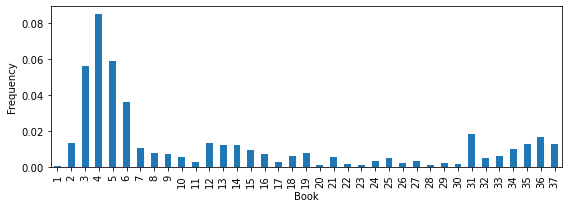
\includegraphics{NHthesis_0728_files/figure-pdf/fig-place_distribution-output-1.png}

}

\caption{\label{fig-place_distribution}Normalized distribution of place
names in \emph{Natural History}}

\end{figure}

\hypertarget{text-source-for-the-study}{%
\subsection{Text source for the study}\label{text-source-for-the-study}}

\emph{Natural History} is originally written in Latin. For the purpose
of this study, an English translation conducted by Henry T. Riley
(1816-1878) and John Bostock (1773-1846), which was first published in
1855, is utilized. The translated text is obtained in a digitized
version from the \href{https://topostext.org/the-project}{TOPOSText
project}, having been sourced from the Perseus Project and governed by a
Creative Commons Attribution-Share-Alike 3.0 U.S. License.

Annotations of people's name, places' name and geographical coordinates
are available together with the text of \emph{Natural History}
(\href{https://topostext.org/work/148}{Book1-11},
\href{https://topostext.org/work/153}{Book12-37}) on
\href{https://topostext.org/the-project}{TOPOSText project}. This
invaluable resource allows for the creation of a dataset that includes
both the textual contents and geographical annotations, which can be
utilized to investigate the distribution of place names in the entire
text and examine the frequencies and patterns of geography-related
content.

The extension of the extracted corpora and the workflow of the
extraction will be further explained in the Methodology chapter
(Section~\ref{sec-methodology}).

\hypertarget{sec-research_question}{%
\section{Research Question}\label{sec-research_question}}

\hypertarget{prominent-mentioned-places-in-natural-history}{%
\subsection{\texorpdfstring{Prominent mentioned places in \emph{Natural
History}}{Prominent mentioned places in Natural History}}\label{prominent-mentioned-places-in-natural-history}}

Based on the geographical annotations in \emph{Natural History} provided
by TOPOSText project, there are 2052 unique places mentioned in
\emph{Natural History}.

The top 20 most frequent place names mentioned (as 1\% of total) in
\emph{Natural History} is shown in Table~\ref{tbl-topplace}.

\hypertarget{tbl-topplace}{}
\begin{longtable}[]{@{}llllll@{}}
\caption{\label{tbl-topplace}Top 20 mentioned place names in Natural
History}\tabularnewline
\toprule\noalign{}
& ToposText\_ID & Place\_Name & Lat & Long & Count \\
\midrule\noalign{}
\endfirsthead
\toprule\noalign{}
& ToposText\_ID & Place\_Name & Lat & Long & Count \\
\midrule\noalign{}
\endhead
\bottomrule\noalign{}
\endlastfoot
1687 & https://topostext.org... & Italy & 40.6000 & 16.30000 & 292 \\
2034 & https://topostext.org... & Rome & 41.8910 & 12.48600 & 269 \\
52 & https://topostext.org... & Egypt & 27.1000 & 30.70000 & 261 \\
82 & https://topostext.org... & India & 30.0000 & 74.00000 & 167 \\
57 & https://topostext.org... & Arabia & 28.0000 & 40.00000 & 123 \\
320 & https://topostext.org... & Syria & 35.5000 & 39.00000 & 109 \\
255 & https://topostext.org... & Cyprus & 35.0000 & 33.00000 & 85 \\
109 & https://topostext.org... & Nile & 30.0918 & 31.23130 & 85 \\
2282 & https://topostext.org... & Alps & 44.1420 & 7.34300 & 82 \\
766 & https://topostext.org... & Sicily & 37.6000 & 14.50000 & 71 \\
275 & https://topostext.org... & Crete & 35.2052 & 25.18360 & 64 \\
7 & https://topostext.org... & Ethiopia & 13.0100 & 35.01000 & 58 \\
417 & https://topostext.org... & Rhodes & 36.4408 & 28.22440 & 56 \\
966 & https://topostext.org... & Athens & 37.9718 & 23.72793 & 56 \\
2043 & https://topostext.org... & Capitol & 41.8933 & 12.48300 & 52 \\
298 & https://topostext.org... & Euphrates & 35.2791 & 40.27080 & 47 \\
2241 & https://topostext.org... & Pontus & 43.5000 & 33.50000 & 47 \\
1839 & https://topostext.org... & Campania & 41.1000 & 14.60000 & 46 \\
1480 & https://topostext.org... & Armenia & 39.7020 & 44.29800 & 45 \\
17 & https://topostext.org... & Red Sea & 19.5000 & 39.00000 & 42 \\
545 & https://topostext.org... & Carthage & 36.8500 & 10.32000 & 42 \\
602 & https://topostext.org... & Cilicia & 37.0100 & 34.01000 & 42 \\
\end{longtable}

The place names referenced in \emph{Natural History} are geographically
mapped, with each location marked on the map using its corresponding
coordinates. A dot is assigned to represent each place, with the size
and color of the dot reflecting the frequency of its mention in the
book. The larger and darker the dot, the more frequently the place is
referenced within the context of Natural History.

An intriguing observation from the output, as depicted in
Figure~\ref{fig-geonamemap_pdf}, is the prominence of India, a region
outside the Mediterranean, despite its high frequency of mentions.

\begin{figure}[H]

{\centering 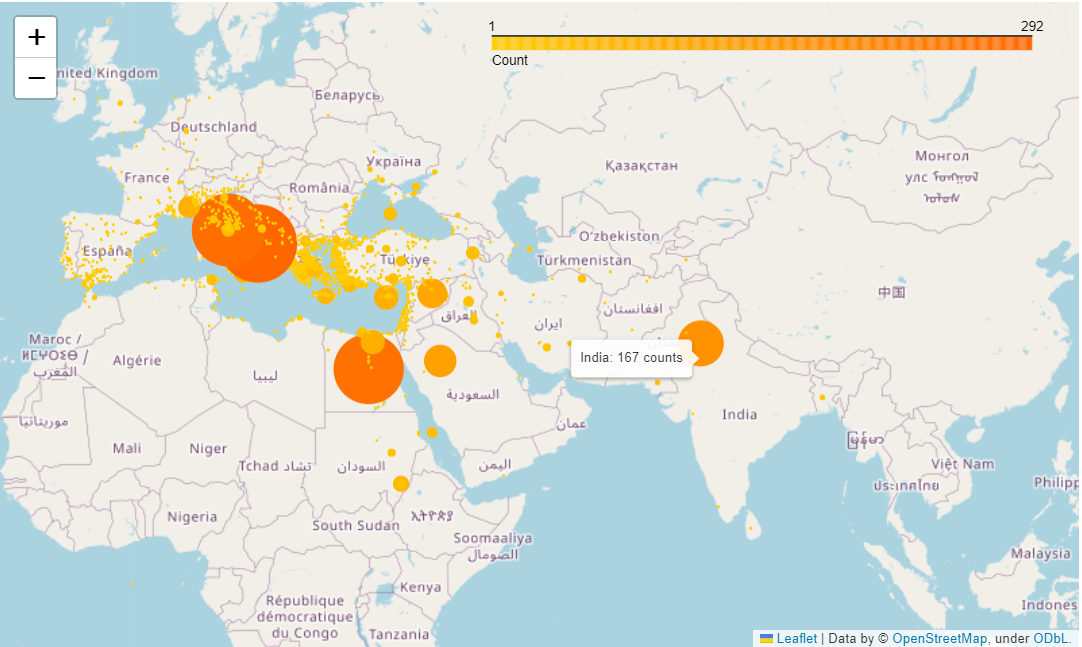
\includegraphics{NHthesis_0728_files/figure-pdf/fig-geonamemap_pdf-output-1.png}

}

\caption{\label{fig-geonamemap_pdf}Place name distribution map}

\end{figure}

\hypertarget{why-india}{%
\subsection{Why India?}\label{why-india}}

Geographically, India presents itself as a distant and disconnected
territory from the Roman Empire, lacking any direct aquatic or land
routes with the Mediterranean region. Despite this apparent physical
separation, the exotic curiosity Pliny attempted to integrate, as well
as the Indo-roman goods exchange network reflected in the work, may
contribute to an explaination of the prominent mentioning of India in
\emph{Natural History} as the broader context.

As suggested by (Murphy 2003), the \emph{mirabilia}, encompassing
accounts of extraordinary landscapes, peoples, plants, and animals,
assumes a substantial proportion within the books of \emph{Natural
History}. Pliny's inclusion of such exotic elements not only catered to
the prevailing curiosity of his Roman readers but also fostered a
comparative perspective between distant locales, exemplified by his
references to India, and their natural counterparts within Rome (Naas
2011). Within research framework of Roman Imperialism, the detailed
portrayal of foreign lands, such as India, holds significant importance
in shaping both Pliny's and his contemporary Roman readers' perception
of their place within the global landscape (Pollard 2009).

In addition, \emph{Natural History} serves as a valuable reference for
tracking the Indo-Mediterranean network of exchange (Pollard 2009).
Through the depiction of cities, ports, and rivers along the trade
routes, the work provides substantive evidence of the flourishing trade
relations between the Roman Empire and the Indian subcontinent (Neelis
2011). The extensive exemplify of diverse commodities, such as
gemstones, glass, spices, textiles, plants, wine, along with the
accounts of the currency \emph{sestertii} involved in the merchandise
exchange in the work shed lights to the compelling details and social
and cultural implications of this long-distance trade (Székely 2006;
Pollard 2009). Furthermore, the direct criticisms regarding the high
cost for the luxury items imported from India implies both the magnitude
of the trade volume and Pliny's stance towards this commercial
interaction (Neelis 2011).

\hypertarget{india-related-text-as-a-case-study}{%
\subsection{India-related text as a case
study}\label{india-related-text-as-a-case-study}}

In light of the observations and foundational research mentioned above,
the present study centers its investigation on the spatial perspective
within Pliny's \emph{Natural History}, with a specific focus on the
texts pertaining to India, seeking to delve into the discourse
surrounding this region. To achieve this goal, distant reading
methodologies, including statistical analysis, topic modeling, and
social network analysis, will be employed.

The main aim of this study is to explore how is India described, and how
is the information about India structured in \emph{Natural History},
which may also contribute to a more profound comprehension of the
inherent complexity and interconnectivity that permeates this monumental
work.

\hypertarget{sec-methodology}{%
\section{Methodology}\label{sec-methodology}}

\hypertarget{workflow}{%
\subsection{Workflow}\label{workflow}}

The workflow for this study involved the following key stages:

\textbf{Data Collection}:

As mentioned in the Introduction chapter
(Section~\ref{sec-introduction}), the text employed for this study is
obtained from the digitized English translation (by Henry T. Riley
(1816-1878) and John Bostock (1773-1846)) of Pliny's \emph{Natural
History} available on \href{https://topostext.org/the-project}{TOPOSText
project}.

The two parts of \emph{Natural History}
(\href{https://topostext.org/work/148}{Book1-11},
\href{https://topostext.org/work/153}{Book12-37}) are scraped for their
the textual contents together with the annotated information of the
geographical coordinates of the ancient places mentioned in the work,
and the book, chapter and paragraph affiliations with the function
provided in
\href{https://www.crummy.com/software/BeautifulSoup/bs4/doc/}{Beautiful
Soup} library of Python.

\textbf{Data Preprocessing}:

The information extracted from the html is structured into separate
columns as \href{https://pandas.pydata.org/}{Pandas} dataframe, a
dataframe for plain text of the entire work, and a dataframe for
geographical-related text in \emph{Natural History} with the
geographical annotations are generated and stored in CSV format
respectively.

After a preliminary exploration, the research focus is narrowed down to
India-related text in \emph{Natural History}. With a reference to the
geographical territories in the consideration of ancient Greek and Roman
world (Talbert 2000b), a dataframe for India-related text is filtered
from the abovementioned dataframe for geographical-related text with the
range of geographical coordinates of India subcontinent in the era of
\emph{Natural History}. The flitered India-related text dataframe is
also stored in CSV format.

The location names mentioned in the India-related text is cross checked
manually. For those have not annotated in the TOPOSText, they are
appended to the dataset.

\textbf{Data Analysis}:

Statistical analysis is conducted in the preliminary exploration of the
extracted dataframes. A nomalized frequency of geographical name
occurence in each book is calculated for an overview of the place name
distribution in \emph{Natural History}. And the top 1\% prominently
mentioned place names in the entire work are sorted out with the time of
their occurencies. The specific attention on India-related text as a
case study is drown from this initial observation.

In the analysis of the India-related text (target corpus) in
\emph{Natural History}, three analysis methods are employed:

\begin{enumerate}
\def\labelenumi{\arabic{enumi}.}
\item
  Word frequency: single word frequency and bi-gram collocation of the
  target corpus are measured with the functions in
  \href{https://www.nltk.org/}{NLTK} package for an overview of the
  keywords relating to India in \emph{Natural History}.
\item
  Topic modelling: \href{https://radimrehurek.com/gensim/}{Genism}
  library is used for semantic vectorization and implemetion of Latent
  Dirichlet Allocation (LDA) model for the topic modelling of the
  India-ralated text, and the library of
  \href{https://pyldavis.readthedocs.io/en/latest/index.htmlgenism}{pyLDAvis}
  is utilized for an interactive visualization. The output of this
  method shows the potential topics in the India-related text in
  \emph{Natural History}.
\item
  Network analysis for Named Entities: Person names mentioned in the
  target corpus are retrieved from the tagging of the text given by the
  pretrained multilingual Named Entity Recognition model
  \href{https://huggingface.co/flair}{Flair}. The person name entities
  are cross checked with the annotation on TOPOSText. Stone names, river
  names, mountain names, person names and the book number are extracted
  as nodes, and the co-occurence between the nodes are calculated as
  edges for network analysis. The output of this method is a graph
  showing the clusters of the nodes in the target corpus, indicating the
  structure of the content related to India in \emph{Natural History}.
\end{enumerate}

\textbf{Interpretation and Conclusion}:

The workflow and parameter setting of each research method is explained
in the beginning of each analysis section. The results aquired from each
method is interpreted with a dialouge to the broader literature and
close reading of the related text.

In the Conclusion chapter, the findings are illustrated comprehensively
in the context of the research questions. And the limitations of each
method is discussed and evaluated.

\hypertarget{data-preparation}{%
\subsection{Data preparation}\label{data-preparation}}

The present section provides an overview of the data preparation
process, encompassing three sub-sections: HTML scraping from TOPOSText,
creation of a filtered dataset of ``India-related text,'' and data
completeness checks. The tools and procedures employed in data
collection and dataset generation for the study are elucidated in the
subsequent content.

\hypertarget{html-scraping-from-topostext}{%
\subsubsection{HTML scraping from
TOPOSText}\label{html-scraping-from-topostext}}

As previously stated, the textual contents of Pliny's \emph{Natural
History} are available on the
\href{https://topostext.org/the-project}{TOPOSText project}, presented
in two distinct parts: \href{https://topostext.org/work/148}{Book1-11},
\href{https://topostext.org/work/153}{Book12-37}. Both parts are
provided in HTML format, offering separate sections of the complete
work.

To extract the relevant data, the
\href{https://www.crummy.com/software/BeautifulSoup/bs4/doc/}{Beautiful
Soup} tool, a Python library renowned for parsing HTML and XML
documents, was employed. This process involved navigating the HTML
structure effectively to retrieve essential information.

The text in the HTML documents is organized into paragraphs, each
uniquely identified by an ``id'' attribute that specifies its
corresponding book, chapter, and paragraph number. For instance, a
typical paragraph has an ``id'' tag as follows:

\textbf{\textless p
id=`urn:cts:latinLit:phi0978.phi001:3.9.7'\textgreater{}}

Utilizing these ``id'' attributes, the paragraphs were meticulously
associated with their respective book, chapter, and paragraph
information.

As a result of this data extraction process, a reference dataset was
obtained, comprising the plain text of \emph{Natural History} divided
into paragraphs, with each paragraph assigned a unique identifier, and
separate columns indicating its affliated book, chapter, and paragraph
number. An illustrative example of the dataset's structure can be
refered as Table~\ref{tbl-dataset_plaintext}.

\hypertarget{tbl-dataset_plaintext}{}
\begin{longtable}[]{@{}lllllll@{}}
\caption{\label{tbl-dataset_plaintext}Example for the reference dataset
containing the plain text in paragraphs of \emph{Natural
History}}\tabularnewline
\toprule\noalign{}
& UUID4 & Reference & Book & Chapter & Paragraph & Text \\
\midrule\noalign{}
\endfirsthead
\toprule\noalign{}
& UUID4 & Reference & Book & Chapter & Paragraph & Text \\
\midrule\noalign{}
\endhead
\bottomrule\noalign{}
\endlastfoot
0 & e9e67565-bb... & urn:cts:lat... & 1 & 1 & 1.0 & PREFACE IN ... \\
1 & 010b853d-b8... & urn:cts:lat... & 1 & 2 & 1.0 & But who cou... \\
2 & 2d10e332-9c... & urn:cts:lat... & 1 & 3 & 1.0 & But if Luci... \\
3 & 113e0b4c-5b... & urn:cts:lat... & 1 & 4 & 1.0 & My own pres... \\
4 & 19115032-9f... & urn:cts:lat... & 1 & 5 & 1.0 & For my own ... \\
\end{longtable}

There are a total of 3493 paragraphs in the English translated version
of \emph{Natural History} used in this study. The extracted text
contains 713300 tokens and 31886 types.\footnote{The token and type
  counts were obtained by excluding punctuation marks.} This reference
dataset has been saved in CSV format for record.

Moreover, the geographical annotations concerning the ancient places
mentioned in the text are labeled with a class attribute denoted as
``place'', exemplified by the following HTML code snippet:

\textbf{\textless a about=``https://topostext.org/place/419125LPal''
class=``place'' lat=``41.8896''
long=``12.4884''\textgreater Palatine\textless/a\textgreater{}}

To compile a comprehensive dataset encompassing all the annotated
ancient places, along with their corresponding geographical coordinates
and contextual information (such as book, chapter, and paragraph
numbers), all annotations under the ``place'' class are extracted. This
dataset enables an analysis of the distribution of place names within
\emph{Natural History}.

As certain places may possess multiple names, ToposText\_ID, which is
the unique identifier assigned to distinct places available on TOPOSText
is also extracted as a reference information. An example of the dataset
presenting the geographical-related text in \emph{Natural History} is
provided in Table~\ref{tbl-dataset_geotext} for reference.

\hypertarget{tbl-dataset_geotext}{}
\begin{longtable}[]{@{}lllllllllll@{}}
\caption{\label{tbl-dataset_geotext}Example for the geographical-related
text dataset}\tabularnewline
\toprule\noalign{}
& UUID4 & ToposText\_ID & Place\_Name & Reference & Lat & Long & Book &
Chapter & Paragraph & Text \\
\midrule\noalign{}
\endfirsthead
\toprule\noalign{}
& UUID4 & ToposText\_ID & Place\_Name & Reference & Lat & Long & Book &
Chapter & Paragraph & Text \\
\midrule\noalign{}
\endhead
\bottomrule\noalign{}
\endlastfoot
0 & bf12... & http... & Academy & urn:... & 37.9920 & 23.7070 & 1 & 8 &
1.0 & For ... \\
1 & f782... & http... & Pala... & urn:... & 41.8896 & 12.4884 & 2 & 5 &
1.0 & For ... \\
2 & a0f9... & http... & Esqu... & urn:... & 41.8950 & 12.4960 & 2 & 5 &
1.0 & For ... \\
3 & b8d8... & http... & Capitol & urn:... & 41.8933 & 12.4830 & 2 & 5 &
1.0 & For ... \\
4 & f81b... & http... & Rome & urn:... & 41.8910 & 12.4860 & 2 & 6 & 3.0
& Belo... \\
\end{longtable}

According to the geographical annotations of the ancient places occured
in \emph{Natural History}, there are 5595 occurences of place names in
book 1-11 and 3281 in book 12-37, adding up to a combined total of 8876
annotated places throughout the work. The geographical-related text in
\emph{Natural History} contains 415474 tokens and 26592
types.\footnote{The token and type counts were obtained by excluding
  punctuation marks.} This dataset including place names and their
textual context in \emph{Natural History} is saved in CSV format for
record.

\hypertarget{filtered-dataset-of-india-related-text}{%
\subsubsection{Filtered dataset of ``India-related
text''}\label{filtered-dataset-of-india-related-text}}

As outlined in the Research Question chapter
(Section~\ref{sec-research_question}), this thesis examines texts
concerning the Indian region in Pliny's \emph{Natural History} as a case
study. The objective is to explore how India is described, portrayed,
and imagined within this extensive work, providing valuable insights
into its complexity.

To ensure a comprehensive contextual analysis, the dataset creation
considers not only instances where the word ``India'' is directly
mentioned but also text related to the Indian region. This broader
approach aims to encompass a wider scope of relevant information.
Drawing from the research and mapping of the Indian region in the
perception of the ancient Greek and Roman world, as explained and
manifested in the \emph{Barrington Atlas of the Greek and Roman World}
(Talbert 2000a, 2000b), the approximate coordinates defining the target
region are as follows\footnote{As indicated in the map-by-map directory,
  the range spans territories of ``modern states of India (minus the
  Punjab), Bangladesh, Bhutan, Burma, Nepal, and Sri Lanka''.}:

\begin{itemize}
\tightlist
\item
  Latitude: 5-35 degrees North
\item
  Longitude: 65-95 degrees East
\end{itemize}

Utilizing the aforementioned dataset of geographical-related text in
\emph{Natural History}, the text having annotations with geographical
coordinates falling within the specified range are extracted to
construct a dataset relevant to the discourse about Indian region in the
work. The filtering process ensures not only the text explicitly
mentioning ``India'' but also those including other place names situated
within the defined boundaries of the Indian region were retained.

The new dataset comprises the textual content as well as the
geographical coordinates of the mentioned Indian place in \emph{Natural
History}. An example of the structure of the dataset of India-related
text is showed as Table~\ref{tbl-dataset_indiatext}.

\hypertarget{tbl-dataset_indiatext}{}
\begin{longtable}[]{@{}lllllllllll@{}}
\caption{\label{tbl-dataset_indiatext}Example for the India-related
dataset}\tabularnewline
\toprule\noalign{}
& UUID4 & ToposText\_ID & Place\_Name & Reference & Lat & Long & Book &
Chapter & Paragraph & Text \\
\midrule\noalign{}
\endfirsthead
\toprule\noalign{}
& UUID4 & ToposText\_ID & Place\_Name & Reference & Lat & Long & Book &
Chapter & Paragraph & Text \\
\midrule\noalign{}
\endhead
\bottomrule\noalign{}
\endlastfoot
85 & 261e... & http... & India & urn:... & 30.0000 & 74.0000 & 2 & 75 &
1.0 & Simi... \\
92 & 5c49... & http... & India & urn:... & 30.0000 & 74.0000 & 2 & 75 &
1.0 & Simi... \\
93 & 9955... & http... & India & urn:... & 30.0000 & 74.0000 & 2 & 75 &
1.0 & Simi... \\
218 & 8199... & http... & Indus & urn:... & 25.4487 & 68.3192 & 2 & 98 &
1.0 & Near... \\
343 & 9a9f... & http... & India & urn:... & 30.0000 & 74.0000 & 2 & 112
& 1.0 & Our ... \\
\end{longtable}

There are 229 occurrences of paragraphs mentioning the places in Indian
region with geographical coordinates annotation. And the distinct places
mentioned are {[}`India' `Indus' `Ganges' `Acesinus' `Hydaspes'
`Taprobane' `Arachosia' `Muziris' `Baragaza' `Ceylon'{]}. The textual
content pertaining India region compiles 37591 tokens and 6048
types.\footnote{The token and type counts were obtained by excluding
  punctuation marks.} The dataset and corpus for India-related text in
\emph{Natural History} are saved respectively in CSV format for further
reference.

\hypertarget{data-completeness-check}{%
\subsubsection{Data completeness check}\label{data-completeness-check}}

The paragraphs extracted from the India-related text dataset undergo
manual verification for the completeness of Indian place name
annotations. Each distinct paragraph in the dataset is individually
extracted and stored in TXT format as separate files within a corpus
folder. The file names contain information about the affiliating book,
chapter, and paragraph numbers.

There are in total 146 distinct paragraghs metioning India places in
\emph{Natural History} accroding to the annotations on TOPOSText.

An example of the exported file name can be referred as follows:

\begin{verbatim}
Exported india_corpus\37.77.1_text.txt
\end{verbatim}

The text files are uploaded to
\href{https://recogito.pelagios.org/}{Recogito} platform, which offers a
semantic annotation tool and automatic geographical annotation
suggestions from its supported gazetteers. This process is used to
cross-check the Indian place name annotations against the data from
TOPOSText. Any unannotated Indian place names are identified and marked
on the \href{https://recogito.pelagios.org/}{Recogito} workspace for
further analysis and evaluation.

\hypertarget{data-analysis}{%
\section{Data Analysis}\label{data-analysis}}

\hypertarget{place-name-distribution-in-india-related-text}{%
\subsection{Place name distribution in India-related
text}\label{place-name-distribution-in-india-related-text}}

The comparison between the total number of place names and the place
names specifically related to the Indian subcontinent mentioned in each
book, is depicted in
Figure~\ref{fig-grouped_place_name_count_comparison}. The difference in
numbers between the two categories is significant, as indicated by the
large disparity.

To facilitate a more effective comparison of the referencing trends
across different books,
Figure~\ref{fig-subplots_place_name_count_comparison} presents subplots
with varying y-axis scales. This approach allows for a clearer
visualization of the trends and patterns in place name references
throughout the various books.

\begin{figure}[H]

{\centering 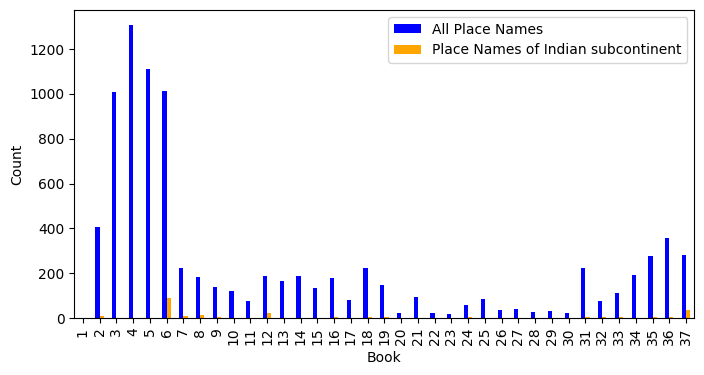
\includegraphics{NHthesis_0728_files/figure-pdf/fig-grouped_place_name_count_comparison-output-1.png}

}

\caption{\label{fig-grouped_place_name_count_comparison}Occurence count
for all place names and place names of Indian subcontinent in each book}

\end{figure}

\begin{figure}[H]

{\centering 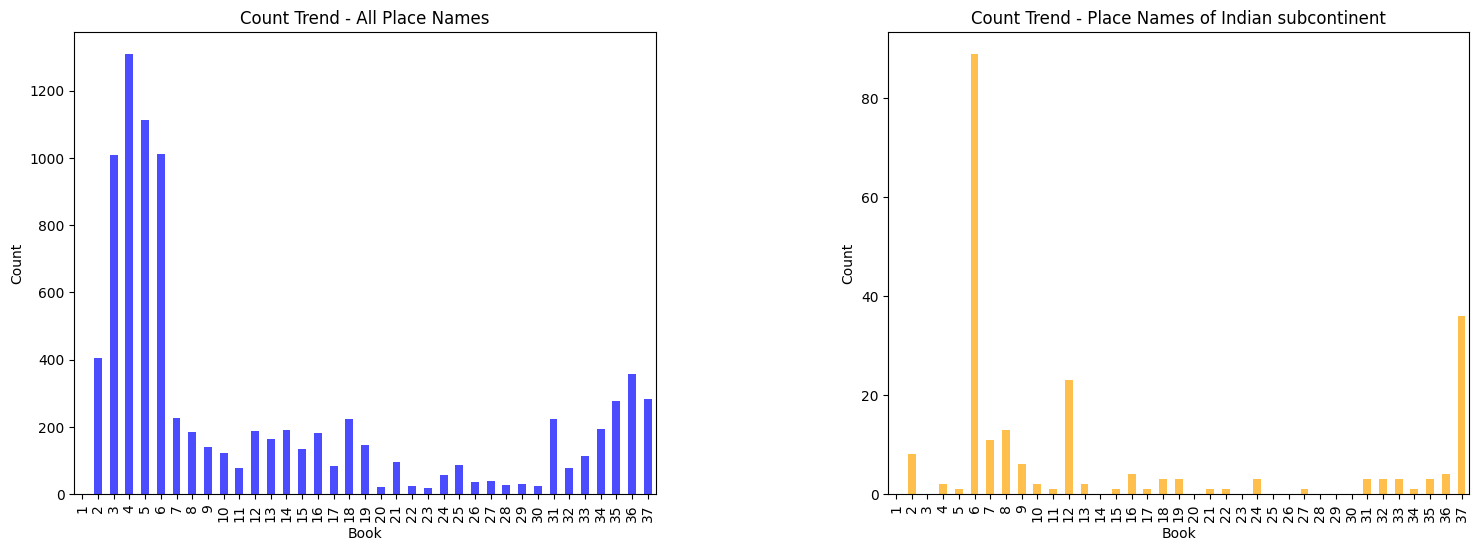
\includegraphics{NHthesis_0728_files/figure-pdf/fig-subplots_place_name_count_comparison-output-1.png}

}

\caption{\label{fig-subplots_place_name_count_comparison}Occurence count
for all place names and place names of Indian subcontinent in each
book\_different y-axis scales}

\end{figure}

The figures reveal a distinct difference between the occurrence trends
of place names related to the Indian subcontinent and all place names
collectively. Specifically, the referencing of the Indian subcontinent
is highly concentrated in books 6, 12, and 37 of Pliny's narrative. This
discrepancy indicates that the mentioning of place names from the Indian
subcontinent is closely tied to specific themes and topics within
Pliny's work.

In this regard, three methodologies have been employed to analyze the
texts pertaining to the Indian subcontinent in \emph{Natural History},
including word frequency and collocation analysis, topic modeling, and
network analysis. The objective of these analyses is to delve deeper
into the textual content, unraveling the intricate relationships and
uncovering the underlying themes and connections associated with the
place names of the Indian subcontinent.

Through word frequency and collocation analysis, the aim is to identify
keyword and significant word combinations co-occur in the textual
content about India in \emph{Natural History}. This analysis provides
insights into the specific linguistic patterns and contextual
associations surrounding the Indian places mentioned in the work,
providing an overview of the keyword in the discourse.

Topic modeling allows for a broader exploration of the thematic
landscape within which the Indian subcontinent place names are embedded.
By clustering related words and identifying prevalent topics, this
methodology helps to discern the major themes and subject matters that
emerge from Pliny's narrative, providing a comprehensive understanding
of the broader context in which these place names are mentioned.

Furthermore, network analysis offers a visual representation of the
interconnections among the place names of the Indian subcontinent and
other entities in Pliny's work. By examining the relationships between
different locations and named entities, this analysis uncovers the
geographical and conceptual networks that exist within the text,
revealing how the Indian subcontinent place names contribute to the
overall structure and narrative flow of \emph{Natural History}.

Together, these methodologies aim to provide a nuanced and comprehensive
exploration of the texts related to the Indian subcontinent in
\emph{Natural History}. By delving into the linguistic, thematic, and
network aspects of these place names, a deeper understanding of their
role in shaping Pliny's narrative can be achieved.

\hypertarget{word-frequency---to-be-re-organized-from-this-part}{%
\subsection{Word frequency - To be re-organized from this
part}\label{word-frequency---to-be-re-organized-from-this-part}}

Through the utilization of measures available in the
\href{https://www.nltk.org/}{NLTK} package, a word frequency list and a
list of collocating bi-grams of the texts pertaining to the Indian
subcontinent are generated to investigate potential keywords and themes
of interest.

To enhance the relevance and descriptive nature of the frequency list,
particular attention has been given to exclude two commonly encountered
but less informative words, namely ``india'' and ``also'', from the
token list.

Among 17661 tokens of the whole corpus for Indian subcontinent related
text, 201 (the top 1\%) frequent words is filterd out and shown in
Figure~\ref{fig-freqwords_treemap} and
Figure~\ref{fig-freqwords_wordcloud}.

\begin{figure}[H]

{\centering 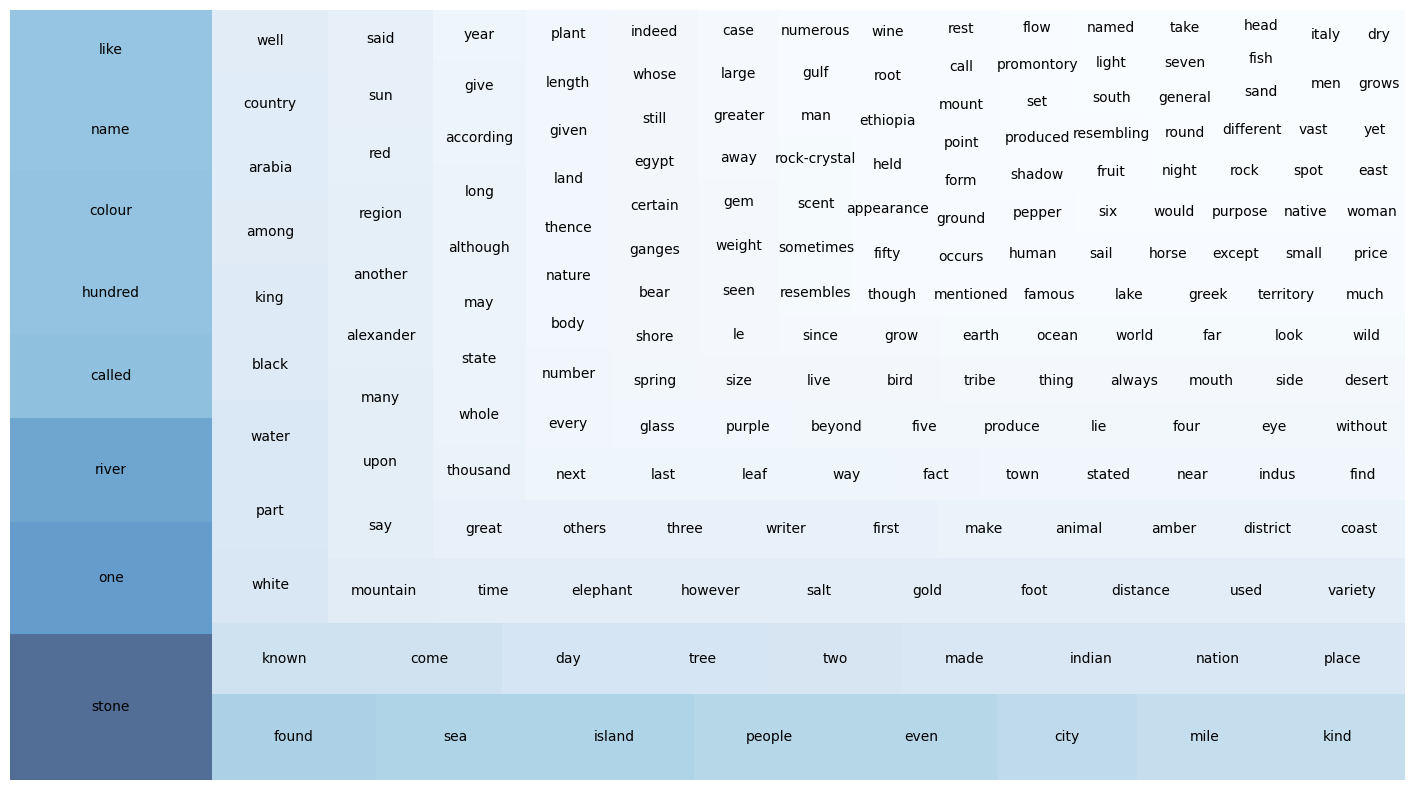
\includegraphics{NHthesis_0728_files/figure-pdf/fig-freqwords_treemap-output-1.png}

}

\caption{\label{fig-freqwords_treemap}Top 1\% frequent words in Indian
subcontinent related text as tree map}

\end{figure}

\begin{figure}[H]

{\centering 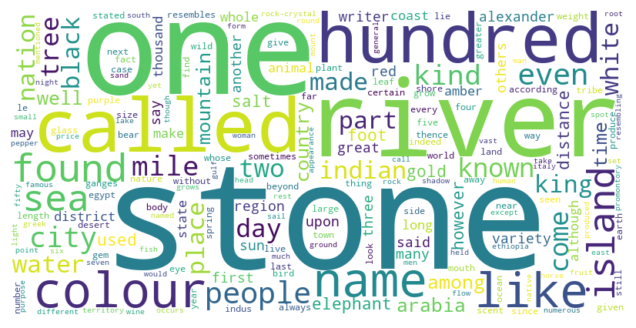
\includegraphics{NHthesis_0728_files/figure-pdf/fig-freqwords_wordcloud-output-1.png}

}

\caption{\label{fig-freqwords_wordcloud}Top 1\% frequent words in Indian
subcontinent related text as word cloud}

\end{figure}

As depicted in the visualizations, the words ``stone,'' ``river,'' and
``color'' notably stand out, suggesting their prominence in the
narrative pertaining to the regions of the Indian subcontinent. This
observation is indicative of the significant references to precious
stones and the origins and transportation routes associated with the
trade of such valuable commodities.

The collocating bi-grams associated with place names of the Indian
subcontinent region are extracted based on the top 20 highest scores in
the likelihood ration measurement. A higher likelihood ratio score
indicates a stronger association or collocation between the words,
suggesting that they are more likely to appear together in the given
text.

The extracted collocations undergo a filtering process that specifically
includes those involving keywords of place names within the regions of
the Indian subcontinent, whihc enables a focused analysis of
collocations directly relevant to the geographic context.

\begin{verbatim}
[('already', 'mentioned'),
 ('present', 'day'),
 ('alexander', 'great'),
 ('father', 'liber'),
 ('taken', 'drink'),
 ('formerly', 'called'),
 ('majesty', 'augustus'),
 ('fifty', 'mile'),
 ('late', 'majesty'),
 ('next', 'come'),
 ('roman', 'citizen'),
 ('mile', 'circumference'),
 ('human', 'being'),
 ('greek', 'name'),
 ('late', 'lamented'),
 ('marcus', 'varro'),
 ('one', 'hundred'),
 ('hundred', 'fifty'),
 ('rising', 'dog-star'),
 ('emperor', 'nero')]
\end{verbatim}

Interestingly, in the flitered bi-grams, 20\% of them are referring to
human names or names of gods in myths (e.g.~Alexander III, the Great
(king of Macedon); Octavius Caesar Augustus (Roman Emperor); Nero (Roman
emperor); Marcus Varro (ancient Latin scholar), Father Liber (referring
to Dionysus, Greek god of winemaking and wine)).

As shown in the quotation of Book 16, Chapter 62, Paragraph 1, the word
``India'' was mentioned in the context of an introduction of a plant, as
a counterpart in the plant origin, and as a conquered land intertwining
with the historical story about how the plant was brought to Rome by
Alexander the Great.

\begin{quote}
16.62.1 It is said that ivy now grows in Asia Minor. Theophrastus about
314 BC. had stated that it did not grow there, nor yet in \textbf{India}
except on Mount Meros, and indeed that Harpalus had used every effort to
grow it in Media without success, while \textbf{Alexander} had come back
victorious from \textbf{India} with his army wearing wreaths of ivy,
because of its rarity, in imitation of \textbf{Father Liber}; and it is
even now used at solemn festivals among the peoples of Thrace to
decorate the wands of that god, and also the worshippers' helmets and
shields, although it is injurious to all trees and plants and
destructive to tombs and walls, and very agreeable to chilly snakes, so
that it is surprising that any honour has been paid to it.
\end{quote}

\#\#(More detailed analysis and illustration will be further conducted
for the pattern of interactions between Indian subcontinent place names
and human names in the book. )

\hypertarget{topic-modelling}{%
\subsection{Topic modelling}\label{topic-modelling}}

Since the corpus size for text pertaining Indian subcontient region is
rather small, with certain tryouts, the the number of topics is set as 3
and the passes is set as 40 to get the most noon-overlapping topic
clusters.

The word ``India'' is excluded from the corpus in order to get more
descriptive keywords which may contribe to a more concrete topic
summary.

The top 30 keywords for each topic, along with their respective weights,
which rank their contributions to the topic is shown and visualized as
follows.

\begin{verbatim}
[(0,
  '0.011*"river" + 0.011*"hundred" + 0.008*"city" + 0.008*"mile" + '
  '0.008*"also" + 0.007*"island" + 0.007*"one" + 0.007*"sea" + 0.006*"nation" '
  '+ 0.005*"come" + 0.005*"called" + 0.005*"people" + 0.004*"distance" + '
  '0.004*"place" + 0.004*"name" + 0.004*"two" + 0.004*"thousand" + '
  '0.004*"alexander" + 0.004*"king" + 0.003*"country" + 0.003*"writer" + '
  '0.003*"upon" + 0.003*"even" + 0.003*"coast" + 0.003*"mountain" + '
  '0.003*"thence" + 0.003*"indus" + 0.003*"elephant" + 0.003*"day" + '
  '0.003*"stated"'),
 (1,
  '0.011*"also" + 0.011*"stone" + 0.006*"like" + 0.006*"colour" + 0.005*"kind" '
  '+ 0.005*"one" + 0.004*"white" + 0.004*"salt" + 0.004*"found" + '
  '0.004*"called" + 0.004*"even" + 0.003*"name" + 0.003*"part" + 0.003*"water" '
  '+ 0.003*"black" + 0.003*"people" + 0.003*"leaf" + 0.003*"made" + '
  '0.003*"foot" + 0.003*"glass" + 0.003*"indian" + 0.003*"arabia" + '
  '0.003*"say" + 0.002*"used" + 0.002*"tree" + 0.002*"time" + 0.002*"among" + '
  '0.002*"plant" + 0.002*"day" + 0.002*"spring"'),
 (2,
  '0.013*"stone" + 0.007*"also" + 0.006*"found" + 0.006*"colour" + '
  '0.006*"like" + 0.006*"one" + 0.005*"name" + 0.005*"amber" + 0.004*"tree" + '
  '0.004*"known" + 0.004*"called" + 0.004*"variety" + 0.003*"river" + '
  '0.003*"even" + 0.003*"gold" + 0.003*"kind" + 0.003*"part" + 0.003*"island" '
  '+ 0.003*"rock-crystal" + 0.002*"many" + 0.002*"sea" + 0.002*"day" + '
  '0.002*"people" + 0.002*"however" + 0.002*"king" + 0.002*"white" + '
  '0.002*"made" + 0.002*"gem" + 0.002*"well" + 0.002*"produce"')]
\end{verbatim}

The three generated topics for the Indian subcontinent related texts can
be summarized based on the dominant words as follows:

Topic 1: \textbf{Stones, Rivers, and Islands} - various elements related
to stones, rivers, and islands. It also touches upon the notion of
distance and the mention of gold and gems.

Topic 2: \textbf{Cities, Trees, and Natural Features} - cities, trees,
and natural features. It also mentions amber, mountains, and the
connection to Arabia.

Topic 3: \textbf{Salt, Sea, and Water} - salt, the sea, and
water-related concepts. It also touches upon topics such as animals,
Alexander the Great, and the notion of a country.

And Topic 1: \textbf{Stones, Rivers, and Islands} takes the forefront
among the other topics.

Consistent with the findings in the frequency list of the corpus, it is
evident that ``stones'' and ``rivers'' hold a significant presence in
the narrative concerning the Indian subcontinent.

\begin{verbatim}
<IPython.core.display.HTML object>
\end{verbatim}

The interactive visualisation of the 3 clusters of the topic modelling
about India-related text can be accessed on the html version of this
\href{https://raw.githack.com/lizaodawn/NH_thesis/main/NHthesis.html}{thesis}.

The static demonstration of the visuslisation can be referred as
Figure~\ref{fig-topic_cluster1}, Figure~\ref{fig-topic_cluster2} and
Figure~\ref{fig-topic_cluster3}.

In the left panel of the above interactive chart, each bubble represents
a topic, and the size of the bulbble indicates the percentage of the
texts in the corpus contributing to the topic. The distance between the
bubbles implies the extent of difference between them. And a good topic
model is expected to have big and non-overlapping bubbles scattered
throughout the chart (Tran 2022).

And in the right panel, the blue bars represent the overall frequency of
each word in the corpus. If no topic is selected, the blue bars of the
most frequently used words will be displayed. When hovering on the
bubbles in the left panel, there will be red bars in the right panel
giving the estimated number of times a given term was generated by a
given topic. The word with the longest red bar is estimated to be used
the most in the texts belonging to that topic.

\begin{figure}[H]

{\centering 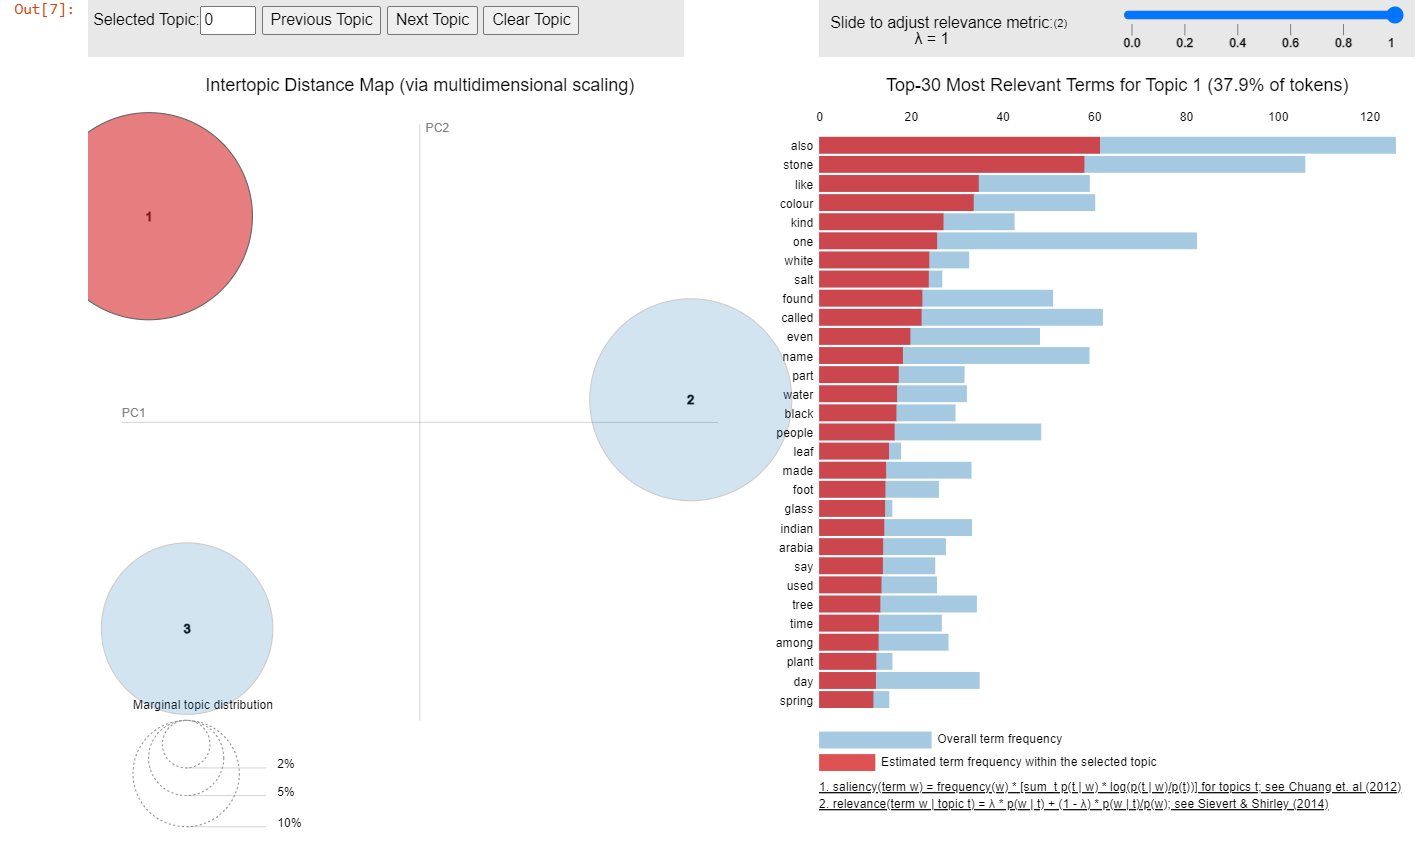
\includegraphics{NHthesis_0728_files/figure-pdf/fig-topic_cluster1-output-1.png}

}

\caption{\label{fig-topic_cluster1}Topic cluster 1}

\end{figure}

\begin{figure}[H]

{\centering 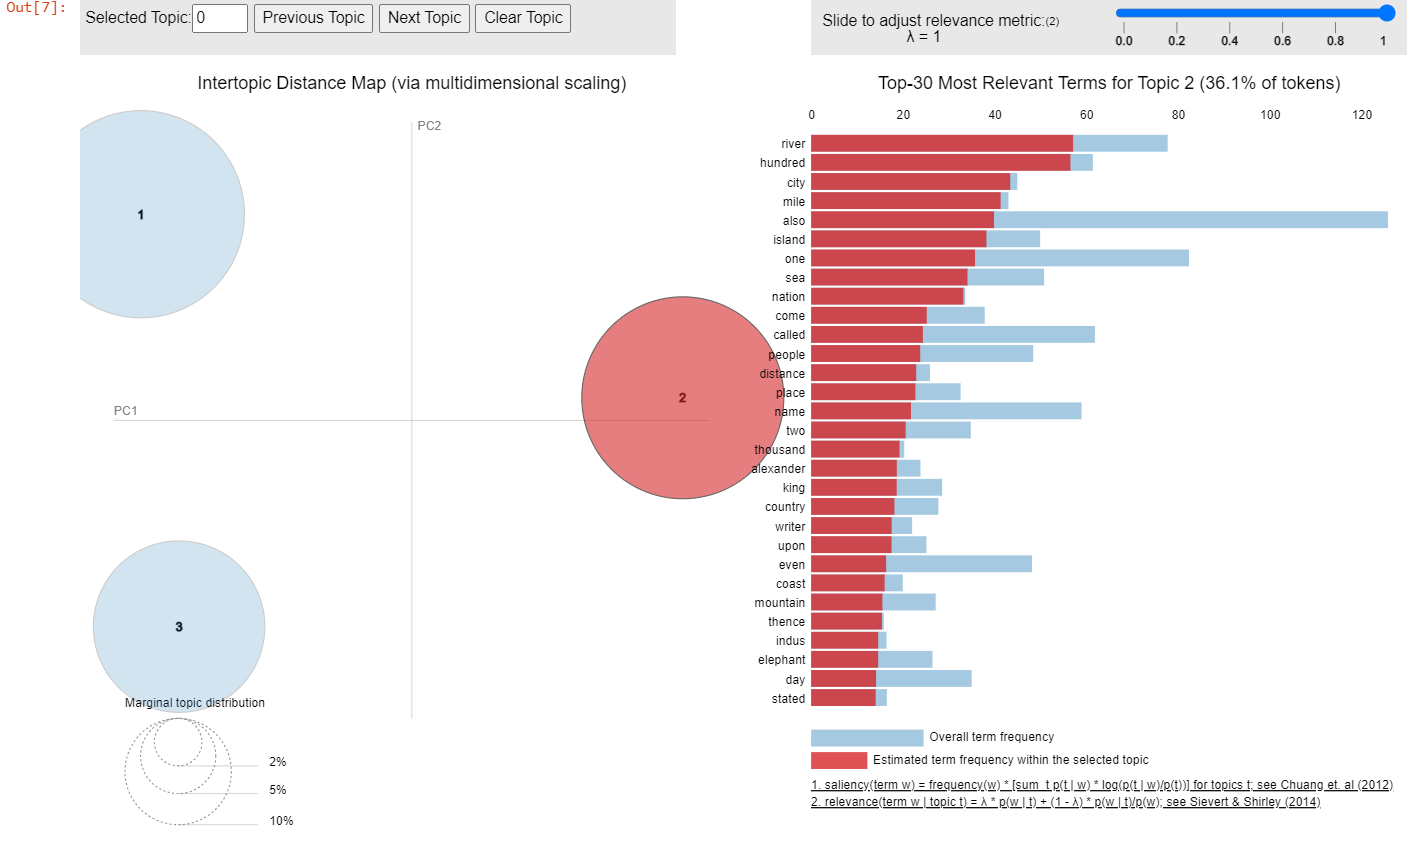
\includegraphics{NHthesis_0728_files/figure-pdf/fig-topic_cluster2-output-1.png}

}

\caption{\label{fig-topic_cluster2}Topic cluster 2}

\end{figure}

\begin{figure}[H]

{\centering 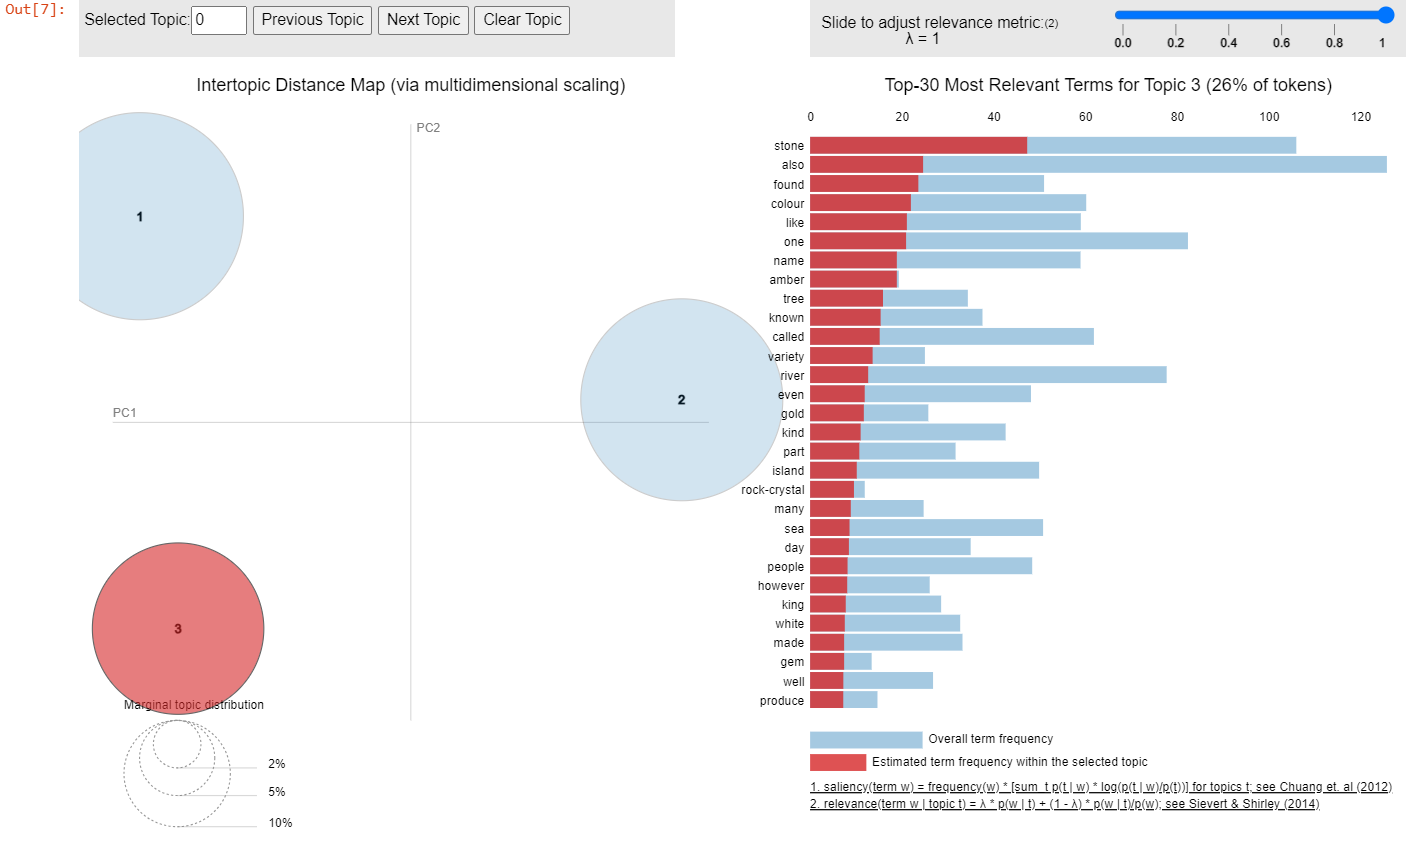
\includegraphics{NHthesis_0728_files/figure-pdf/fig-topic_cluster3-output-1.png}

}

\caption{\label{fig-topic_cluster3}Topic cluster 3}

\end{figure}

\hypertarget{network-analysis-for-named-entities}{%
\subsection{Network analysis for named
entities}\label{network-analysis-for-named-entities}}

\hypertarget{conclusions}{%
\section{Conclusions}\label{conclusions}}

\{\#refs\}

\hypertarget{refs}{}
\begin{CSLReferences}{1}{0}
\leavevmode\vadjust pre{\hypertarget{ref-beagon2011}{}}%
Beagon, Mary. 2011. {``Chapter {Five}. {The} {Curious} {Eye} {Of} {The}
{Elder} {Pliny}.''} In \emph{Pliny the {Elder}: {Themes} and
{Contexts}}, 71--88. Brill.
\url{https://brill.com/display/book/edcoll/9789004210073/Bej.9789004202344.i-248_006.xml}.

\leavevmode\vadjust pre{\hypertarget{ref-fantoli2022}{}}%
Fantoli, Margherita. 2022. {``Statistics and Linguistics: Can We Tell
Something More about {Pliny} the {Elder}?''}
\url{https://classics-at.chs.harvard.edu/statistics-and-linguistics-can-we-tell-something-more-about-pliny-the-elder/}.

\leavevmode\vadjust pre{\hypertarget{ref-healy1999}{}}%
Healy, John F. 1999. \emph{Pliny the {Elder} on Science and Technology}.
Oxford: university press.

\leavevmode\vadjust pre{\hypertarget{ref-lao2016}{}}%
Lao, Eugenia. 2016. {``Taxonomic {Organization} in {Pliny}'s {Natural}
{History}.''} In \emph{Greek and {Roman} Poetry, the {Elder} {Pliny}},
edited by Francis Cairns and Roy Gibson, 209--46. Papers of the
{Langford} {Latin} {Seminar} 16. Prenton: Francis Cairns Publications.

\leavevmode\vadjust pre{\hypertarget{ref-murphy2003}{}}%
Murphy, Trevor. 2003. {``11. Pliny{'}s Naturalis Historia: The Prodigal
Text.''} In, 301--22. BRILL.
\url{https://doi.org/10.1163/9789004217157_012}.

\leavevmode\vadjust pre{\hypertarget{ref-naas2002}{}}%
Naas, Valérie. 2002. \emph{Le Projet Encyclopédique de {Pline}
l'{Ancien}}. Collection de l'école Française de {Rome} 303. Rome: Ecole
française de Rome.

\leavevmode\vadjust pre{\hypertarget{ref-naas2011}{}}%
---------. 2011. {``Chapter {Four}. {Imperialism}, {Mirabilia}, {And}
{Knowledge}: {Some} {Paradoxes} {In} {The} {Naturalis} {Historia}.''} In
\emph{Pliny the {Elder}: {Themes} and {Contexts}}, 57--70. Brill.
\url{https://brill.com/display/book/edcoll/9789004210073/Bej.9789004202344.i-248_005.xml}.

\leavevmode\vadjust pre{\hypertarget{ref-neelis2011}{}}%
Neelis, J. 2011. {``Chapter {Three}. {Trade} {Networks} {In} {Ancient}
{South} {Asia}.''} In \emph{Early {Buddhist} {Transmission} and {Trade}
{Networks}}, 183--228. Brill.
\url{https://brill.com/display/book/9789004194588/Bej.9789004181595.i-372_004.xml}.

\leavevmode\vadjust pre{\hypertarget{ref-pinkster2005}{}}%
Pinkster, Harm. 2005. {``The {Language} of {Pliny} the {Elder}.''}
\emph{Journal of Asthma - J ASTHMA} 129 (November): 239--56.
\url{https://doi.org/10.5871/bacad/9780197263327.003.0011}.

\leavevmode\vadjust pre{\hypertarget{ref-pollard2009}{}}%
Pollard, Elizabeth Ann. 2009. {``Pliny's {Natural} {History} and the
{Flavian} {Templum} {Pacis}: {Botanical} {Imperialism} in
{First}-{Century} {C}. {E}. {Rome}.''} \emph{Journal of World History}
20 (3): 309--38. \url{https://www.jstor.org/stable/40542802}.

\leavevmode\vadjust pre{\hypertarget{ref-roller2022}{}}%
Roller, D. W. 2022. {``Introduction.''} In \emph{A {Guide} to the
{Geography} of {Pliny} the {Elder}}, 1--14. Cambridge: Cambridge
University Press. \url{https://doi.org/10.1017/9781108693660.003}.

\leavevmode\vadjust pre{\hypertarget{ref-rydberg-cox2021}{}}%
Rydberg-Cox, Jeff. 2021. {``Modeling the {Sources} and {Topics} of
{Pliny}'s {Natural} {History}.''} \emph{Umanistica Digitale}, no. 11:
217--29. \url{https://doi.org/10.6092/issn.2532-8816/12521}.

\leavevmode\vadjust pre{\hypertarget{ref-schultze2011}{}}%
Schultze, Clemence. 2011. {``Chapter {Ten}. {Encyclopaedic}
{Exemplarity} {In} {Pliny} {The} {Elder}.''} In \emph{Pliny the {Elder}:
{Themes} and {Contexts}}, 167--86. Brill.
\url{https://brill.com/display/book/edcoll/9789004210073/Bej.9789004202344.i-248_011.xml}.

\leavevmode\vadjust pre{\hypertarget{ref-szekely2006}{}}%
Székely, Melinda. 2006. {``Eastern {Trade} of the {Roman} {Empire} Based
on {Pliny} the {Elder}'s {Natural} {History}.''} \emph{Chronica} 6
(January): 199--206.
\url{https://www.proquest.com/docview/2379648941/citation/93A42D142D614235PQ/1}.

\leavevmode\vadjust pre{\hypertarget{ref-talbert2000-1}{}}%
Talbert, Richard J. A. 2000a. \emph{Barrington Atlas of the {Greek} and
{Roman} World: Map-by-Map Directory}. Princeton (N.J.): Princeton
university press.

\leavevmode\vadjust pre{\hypertarget{ref-talbert2000}{}}%
---------. 2000b. \emph{Barrington Atlas of the {Greek} and {Roman}
World.} Princeton (N.J.): Princeton university press.

\leavevmode\vadjust pre{\hypertarget{ref-tran2022}{}}%
Tran, Khuyen. 2022. {``pyLDAvis: Topic Modelling Exploration Tool That
Every NLP Data Scientist Should Know.''}
\url{https://neptune.ai/blog/pyldavis-topic-modelling-exploration-tool-that-every-nlp-data-scientist-should-know}.

\end{CSLReferences}



\end{document}
